%
%   Dr.HD
%   "robocon.tex"
%

\documentclass[10pt,b5paper,papersize,dvipdfmx]{jsbook}

\usepackage{vuccaken}
\usepackage{vuccaken2019}

% スタイルファイルの読み込みや自作マクロは, 
% 最終的には vuccaken2019.sty の中に書いてください. 
% とりあえずはここに書いてもらって構いません. 

\begin{document} % 以下本文

\mokuji{2} % 目次出力

% - - - - - - - - - - - - - - - - - - - - - - - - %
\kaishititle%
  {ロボットアーム設計の為の基礎計算}% title
  {ロボティクス学科4回生}% 所属
  {阿部龍幸}% name
% - - - - - - - - - - - - - - - - - - - - - - - - %

\begin{figure}[htbp]
  \centering
  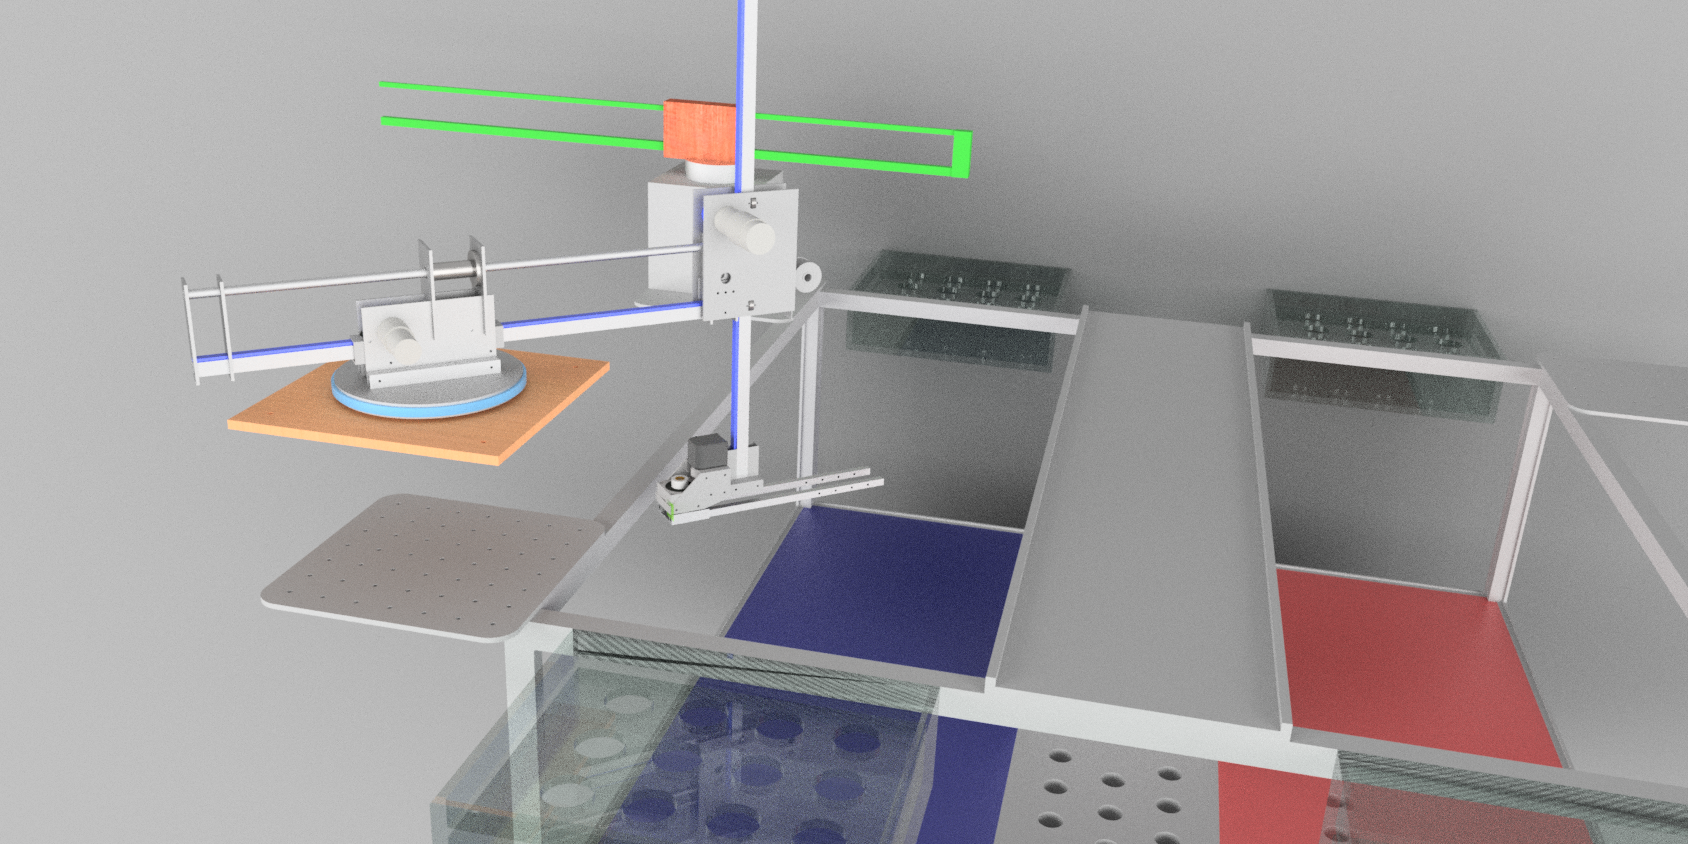
\includegraphics[width=12cm]{robocon/robot_and_field.png}
  % \caption{$y=\sin x$のグラフ. gnuplotで作成した. }
  % \label{fig:robot_and_fields}
\end{figure}

%
\section*{はじめに}
% 会誌ではjsbookクラスを使います. \par
% テーマが複数ある場合は別ファイルで提出してください. 
自分が製作予定のロボットアームの最も肝心な一部分の設計をコンピュータによる解析を用いて行う. この設計では, 使用する材質の強度等を考慮しながらアームの形状を変更し, ロボットがユーザの要求する速度を満たすことを目指す. ロボットをCADソフトで設計する際には, 入手可能な材料を以て製作可能な形状を考慮しつつ, 計算に手間のかからない単純な形状を組み合わせたモデルになるように進める. 以下, 物理量をSI単位系で示し, 有効数字を小数点以下2桁とする. 尚, モデルの画像において寸法の表記は[mm]表記とする. 

%
\section{課題設定}
% はじめにこのファイルのソースを自分のtexファイルにコピペしてください. \par
% figureのパスには注意してください. 
\subsection{設計目的}
包装されたお菓子などの軽量なワークを素早くハンドリングするロボットアームの, ロボットベースに対して垂直にとった軸周りに素早く回転するアーム部分を設計したい. 回転軸周りのトルク$\tau =1.0 \times 10^3 \tani*{Nm}$とし, 重力方向の最大変位を$1.0 \times 10^{-2} \tani*{m}$以下に抑えることを目指して設計する. また, アームの先には, 実際に製作するロボットが備える機構とハンドを簡略化し,$2.0 \tani*{kg}$の荷重がかかるパーツを接続する.
\subsection{使用材料}
アームに使用する材料はアルミ合金とする. 主に用いるアルミは6000系で, 押し出し加工性に優れ, 強度が良好で軽量であるという特徴を持つ. これは設計目的にある素早く動くという要求を慣性モーメントの小ささで満たし, 重力方向の最大変位を抑えるという要求を縦弾性係数が満たすと期待できるからである. 他にも板材として2000系アルミ合金を用いるが, 6000系アルミ合金に比べて強度が高く, 使用する部分の殆どが回転軸に近い場所であり慣性抵抗の違いが小さく, また6000系アルミ合金を長手方向に渡って非常に多く使うのでそのひずみの様子重要視したいという理由で今回は全体を6000系アルミとしてモデルを簡単にして計算する. 以降, 密度$\rho=2.70\times 10^{-6}\tani*{kg/mm^3}$, 縦弾性係数$E=68.90 \tani*{GPa}$, 許容最大応力を$\sigma=2.75×10^{5} \tani*{MPa}$とする. 安全率はこのアームがロボットの最も基にあり衝撃が加わる可能性がある箇所なので, 余裕を見て$f=15.00$とする.
\subsection{座標系}\label{座標系}
基準座標系をロボットベースの底面とし, リンク座標系を円筒状面の中心に設け, 手先座標系はリンクの先端中央部とし, 解析を行う. 参考となるロボットの構造を図\ref{fig:座標系}に示す. 
\begin{figure}[htbp]
  \centering
  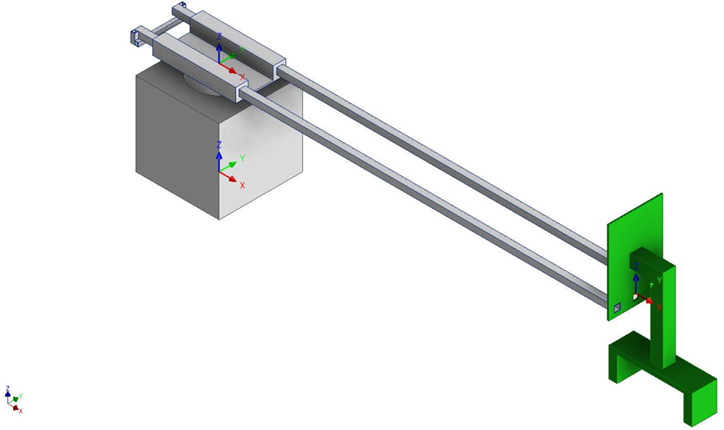
\includegraphics[width=12cm]{robocon/robot01.png}
  \caption{座標系}
  \label{fig:座標系}
\end{figure}
\subsection{基準}\label{基準}
ロボットベースは, 1辺$2.00\times10^{-1} \tani*{m}$の立方体に直径$1.20\times10^{-1} \tani*{m}$で,$z$軸方向に上面から$7.00\times10^{-2} \tani*{m}$の深さの円筒を切り抜いた形状のものとする. 形状を図\ref{fig:ロボットベース}に示す. 
ロボットアームの, ロボットベースの円筒状の中心から手先までの距離については$1.0\tani*{m}$に固定とし, ロボットハンドとジョイントの形状はロボットアームに合わせて変更する. また, ジョイントの重量は無視し, ハンドの重量は$2.0\tani*{kg}$で固定とする. 
ベースとアームを接続するジョイント, ロボットアーム, ロボットハンドの形状については複雑であるので, それぞれ図\ref{fig:ジョイント}, 図\ref{fig:ロボットアーム}, 図\ref{fig:ロボットハンド}に必要な寸法を示す.
\begin{figure}[H]
  \centering
  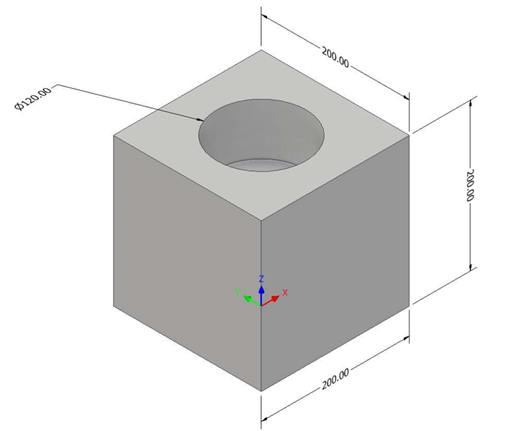
\includegraphics[width=11cm]{robocon/robot02.png}
  \caption{ロボットベース}
  \label{fig:ロボットベース}
\end{figure}
\begin{figure}[H]
  \centering
  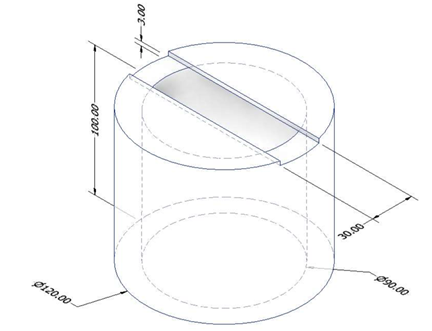
\includegraphics[width=12cm]{robocon/robot03.png}
  \caption{ジョイント}
  \label{fig:ジョイント}
\end{figure}
\begin{figure}[H]
  \centering
  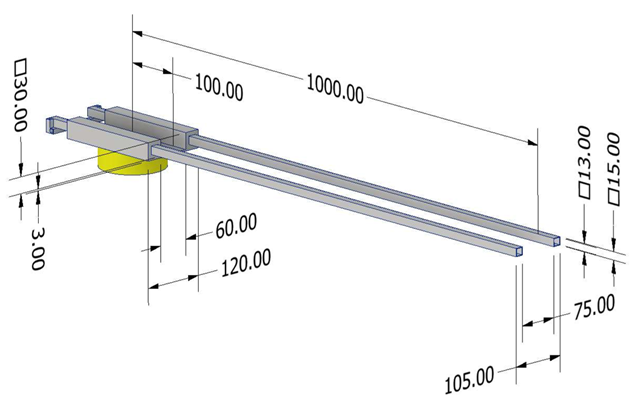
\includegraphics[width=10cm]{robocon/robot04.png}
  \caption{ロボットアーム}
  \label{fig:ロボットアーム}
\end{figure}
\begin{figure}[H]
  \centering
  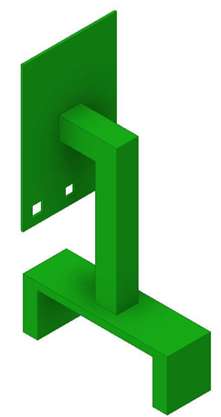
\includegraphics[height=4cm]{robocon/robot05.png}
  \caption{ロボットハンド}
  \label{fig:ロボットハンド}
\end{figure}
このロボットアームを機構解析した結果, \ref{座標系}項で定義した手先座標系に関する手先角加速度, 手先角速度, 手先角度変化, 手先加速度が以下の図\ref{Basic Arm 手先角加速度}から図\ref{fig:Basic Arm 手先加速度}までのグラフに示すように得られた. 
また, 構造解析結果として,最大主応力 , 最大フォンミーゼス応力, 変位が図\ref{fig:Basic Arm 最大主応力}, 図\ref{fig:Basic Arm 最大フォンミーゼス応力}, 図\ref{fig:Basic Arm 変位}のように得られた. 
数値をまとめて表\ref{tbl:Basic Arm 解析結果}に示す.

\begin{table}[H]
  \centering
  \caption{Basic Arm 解析結果}
  \label{tbl:Basic Arm 解析結果}
  \begin{tabular}{|c|c|c|c|c|} \hline
  質量$M\tani*{kg}$& \begin{tabular}{c}角加速度\\$\ddot{q}$$\tani*{rad/s^2}$\end{tabular}& 加速度$\dot{q}$$\tani*{m/s}$& 最大主応力$\sigma\tani*{Pa}$& 変位$\delta_z\tani*{m}$\\ \hline
$1.82$&$4.29\times 10^{-1}$&$4.29\times 10^{-1}$&$7.71\times 10^6$&$1.25\times 10^{-2}$\\ \hline
  \end{tabular}
\end{table}

\begin{figure}[htbp]]
  \centering
  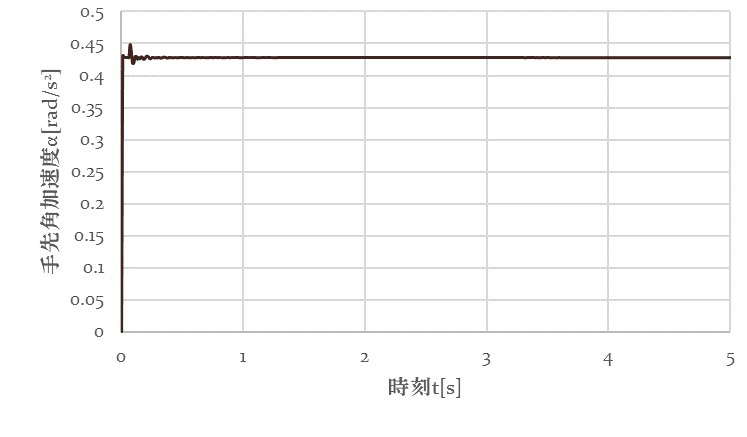
\includegraphics[width=12.6cm]{robocon/robot06.png}
  \caption{Basic Arm 手先角加速度}
  \label{Basic Arm 手先角加速度}
\end{figure}
\begin{figure}[htbp]
  \centering
  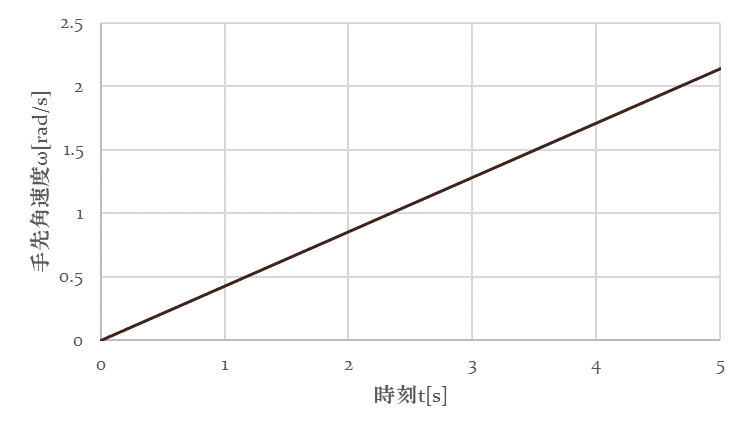
\includegraphics[width=12cm]{robocon/robot07.png}
  \caption{Basic Arm 手先角速度}
  \label{fig:Basic Arm 手先角速度}
\end{figure}
\begin{figure}[htbp]
  \centering
  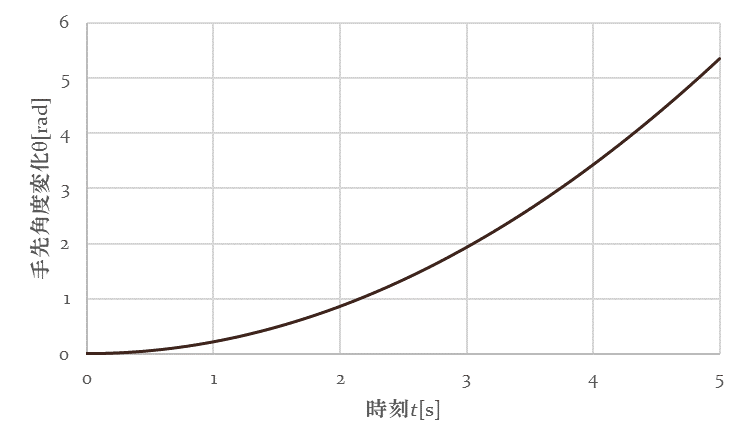
\includegraphics[width=12cm]{robocon/robot08.png}
  \caption{Basic Arm 手先角度変化}
  \label{fig:Basic Arm 手先角度変化2}
\end{figure}
\begin{figure}[htbp]
  \centering
  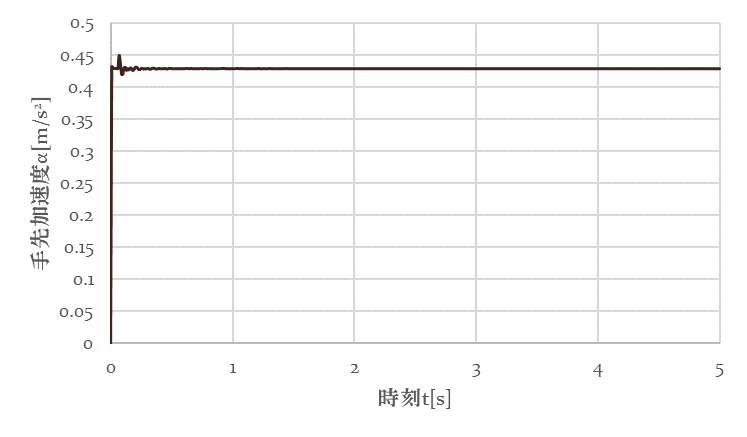
\includegraphics[width=12cm]{robocon/robot09.png}
  \caption{Basic Arm 手先加速度}
  \label{fig:Basic Arm 手先加速度}
\end{figure}
\begin{figure}[htbp]
  \centering
  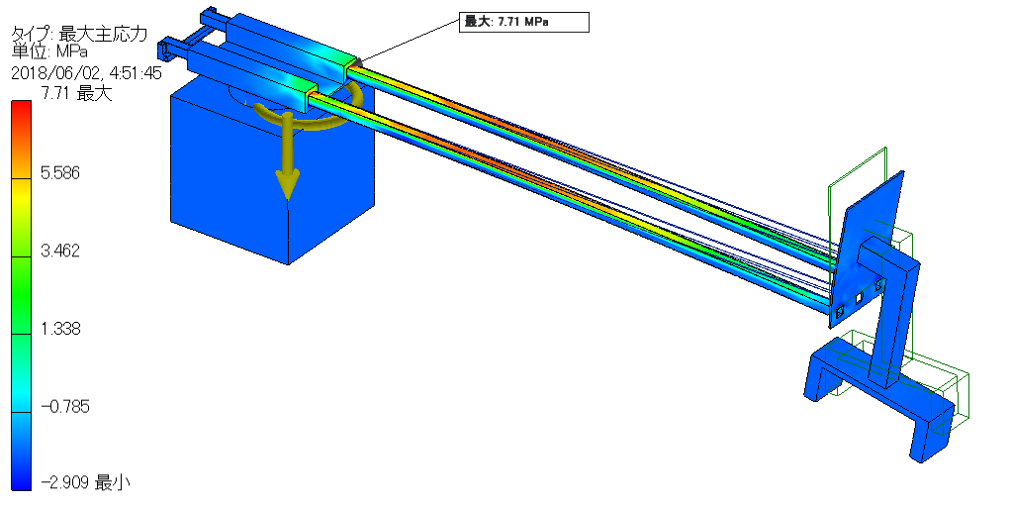
\includegraphics[width=12cm]{robocon/robot10.png}
  \caption{Basic Arm 最大主応力}
  \label{fig:Basic Arm 最大主応力}
\end{figure}
\begin{figure}[htbp]
  \centering
  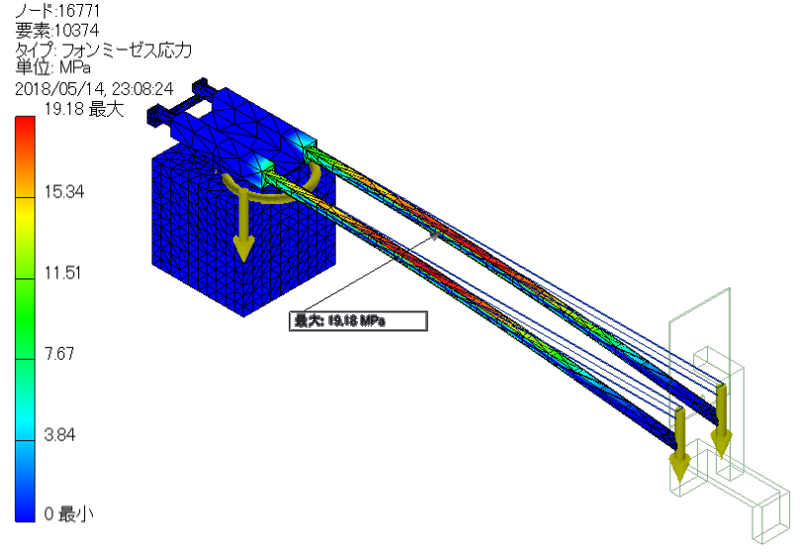
\includegraphics[width=12cm]{robocon/robot11.png}
  \caption{Basic Arm 最大フォンミーゼス応力}
  \label{fig:Basic Arm 最大フォンミーゼス応力}
\end{figure}
\begin{figure}[htbp]
  \centering
  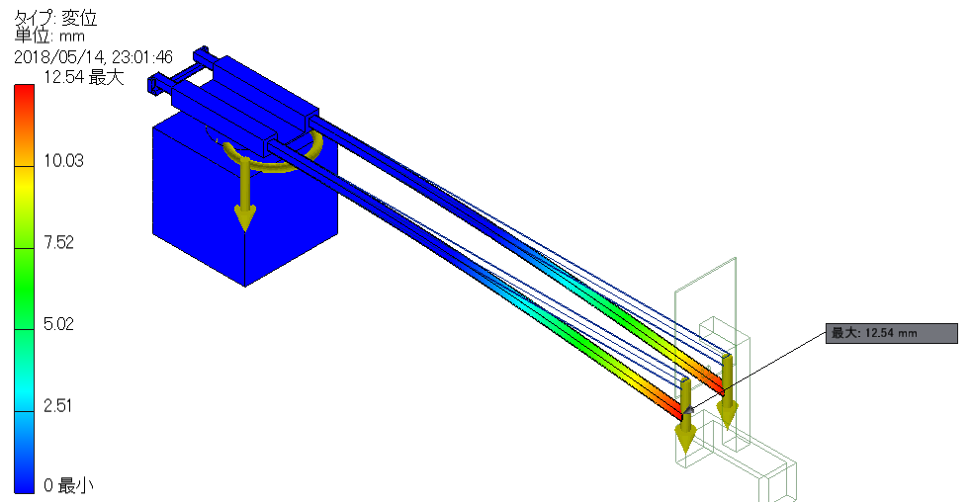
\includegraphics[width=12cm]{robocon/robot12.png}
  \caption{Basic Arm 変位}
  \label{fig:Basic Arm 変位}
\end{figure}
\clearpage
\section{設計}
\subsection{数式}\label{数式}
この項には, 以降の設計過程に必要な理論解を求めるための式を示す. 初めに, 高速性の追求について, 手先角加速度$\ddot{q}$, 最大トルク$\tau_{\mathrm{max}}$, 慣性モーメント$I$とすると, 手先角加速度は以下のような式で表せる.
\begin{align}
\ddot{q}=\frac{\tau_{\mathrm{max}}}{I}
\end{align}
また, 手先加速度$\ddot{r}$はリンク長さ$l$を用いて次のように表せる.
\begin{align}
\ddot{r}=l\ddot{q}
\end{align}
次に応力に関して, 質量$M$, 密度$\rho$, 幅$b$, 高さ$h$, リンク長さ$l$, 回転軸からリンク中心の長さ$x$の直方体リンクにおいて, 慣性モーメントが以下のように与えられる.
\begin{eqnarray}
  I&=&\frac{1}{12}M(l^2+b^2)+Mx^2\\
  &=&\frac{1}{12} \rho lbh(l^2+b^2 )+\rho lbhx^2
\end{eqnarray}
またこの時, 断面係数$Z$は断面係数次のようになる.
\begin{align}
  Z=\frac{1}{6}bh^2
\end{align}
そして外力$F_z$を与えた時の最大応力$\sigma_f$は次のようになる.
\begin{align}
  \sigma_f=\frac{F_zl}{Z}
\end{align}
この時, 安全率$f$, 材質から与えられる許容最大応力$\sigma_A$とで与えられる強度の条件は次のようになる.
\begin{align}
  \sigma_f\leq\frac{\sigma_A}{f}
\end{align}
以降では, 基本的にこれらの式を用いて, 理論的解析を行うものとする.


\subsection{リンク形状の変更}
まず, 基準としたロボットアームが最大変位の要求を満たさなかったので, 高剛性な形に変更し, そこからさらに高速化を目指して変更していくことを考える. アーム先端までの長さについては\ref{基準}項で定めているので変更はせず, 現在のアームを2段重ねにしたような形状に変更する. 詳細の寸法については複雑であるので, 具体的な形状と共に図\ref{fig:Harder Arm}に示す. このリンクの各パラメータについて表\ref{tbl:Harder Arm パラメータ}にまとめた. また, \ref{数式}項の数式を用いて求めた結果を表\ref{tbl:各理論値}にまとめる.
\begin{table}[H]
  \centering
  \caption{Harder Arm パラメータ}
  \label{tbl:Harder Arm パラメータ}
  \begin{tabular}{|c|c|c|} \hline
    リンク長さ$l\tani*{kg}$& 角柱状部分幅$b\tani*{m}$& 角柱状部分高さ$h\tani*{m}$\\ \hline
$1.00$&$1.05\times 10^{-1}$&$0.98\times 10^{-1}$\\ \hline
  \end{tabular}
\end{table}
\begin{table}[H]
  \centering
  \caption{各理論値}
  \label{tbl:各理論値}
  \begin{tabular}{|c|c|c|c|c|} \hline
    質量$M\tani*{kg}$& \begin{tabular}{c}角加速度\\$\ddot{q}$$\tani*{rad/s^2}$\end{tabular}& 加速度$\dot{q}$$\tani*{m/s}$& \begin{tabular}{c}最大応力\\$\sigma\tani*{Pa}$\end{tabular}& \begin{tabular}{c}慣性モーメント\\$I_z\tani*{kgm^2}$\end{tabular}\\ \hline
$2.87$&$3.01\times 10^{-13}$&$3.01\times 10^{-13}$&$1.92\times 10$&$3.32\times 10^{15}$\\ \hline
  \end{tabular}
\end{table}

\begin{figure}[htbp]
  \centering
  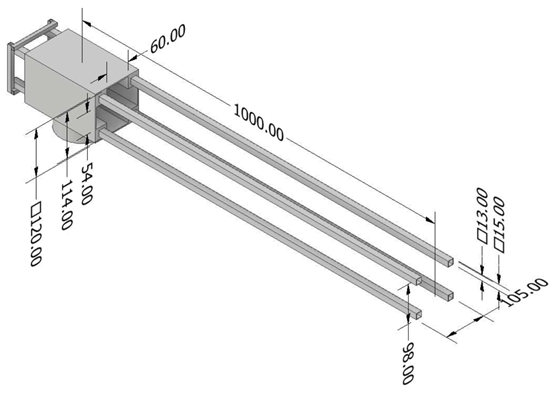
\includegraphics[width=10cm]{robocon/robot13.png}
  \caption{Harder Arm}
  \label{fig:Harder Arm}
\end{figure}

このロボットアームを機構解析した結果, アーム先端に設定した手先座標系に関する手先角加速度, 手先角速度, 手先角度変化, 手先加速度が以下の図\ref{fig:Harder Arm 手先角加速度}から\ref{fig:Harder Arm 手先加速度}までのグラフに示すように得られた. また, 構造解析結果として, 最大主応力, 最大フォンミーゼス応力, 変位が図\ref{fig:Harder Arm 最大主応力}, \ref{fig:Harder Arm 最大フォンミーゼス応力}, \ref{fig:Harder Arm 変位} のように得られた. 数値をまとめて表\ref{tbl:Harder Arm 解析結果}に示す.
\begin{table}[htbp]
  \centering
  \caption{Harder Arm 解析結果}
  \label{tbl:Harder Arm 解析結果}
  \begin{tabular}{|c|c|c|c|c|} \hline
    質量$M\tani*{kg}$& 角加速度$\ddot{q}$$\tani*{rad/s^2}$& 加速度$\dot{q}$$\tani*{m/s}$& 最大応力$\sigma\tani*{Pa}$& 変位$\delta_z\tani*{m}$\\ \hline
    $3.40$&$4.09\times 10^{-1}$&$4.09\times 10^{-1}$&$3.62\times 10^6$&$9.23\times 10^{-4}$\\ \hline
  \end{tabular}
\end{table}

\begin{figure}[htbp]
  \centering
  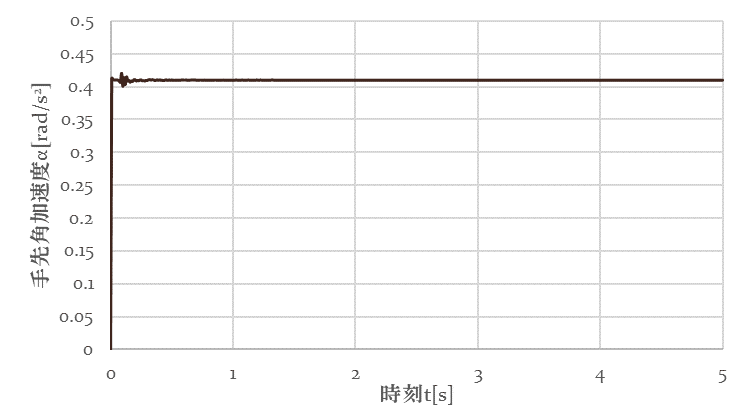
\includegraphics[width=12cm]{robocon/robot14.png}
  \caption{Harder Arm 手先角加速度}
  \label{fig:Harder Arm 手先角加速度}
\end{figure}
\begin{figure}[htbp]
  \centering
  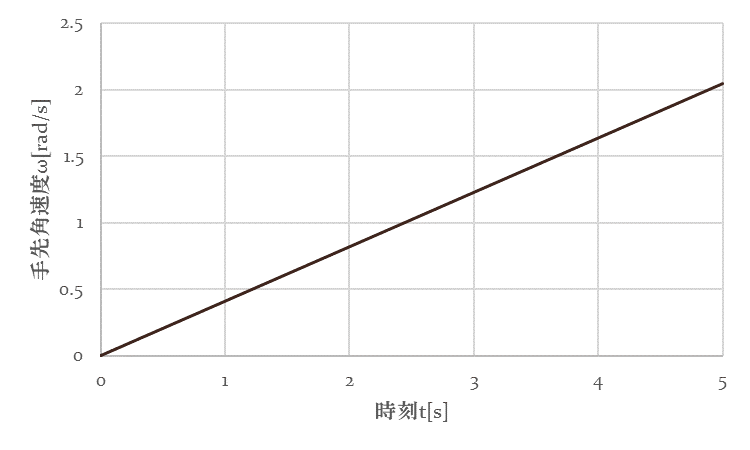
\includegraphics[width=12cm]{robocon/robot15.png}
  \caption{Harder Arm 手先角速度}
  \label{fig:Harder Arm 手先角速度}
\end{figure}
\begin{figure}[htbp]
  \centering
  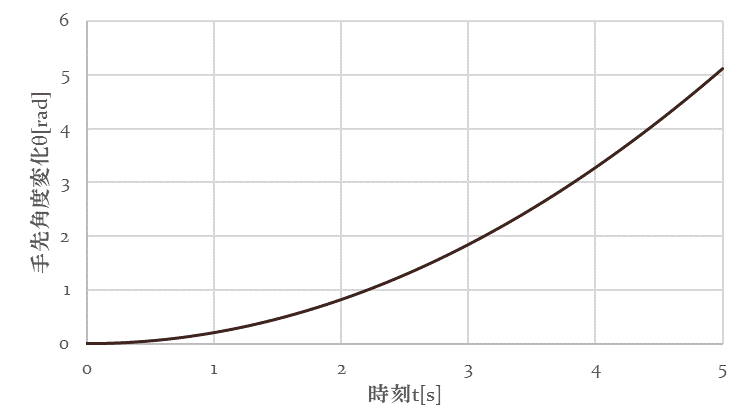
\includegraphics[width=12cm]{robocon/robot16.png}
  \caption{Basic Arm 手先角度変化}
  \label{fig:Basic Arm 手先角度変化}
\end{figure}
\begin{figure}[htbp]
  \centering
  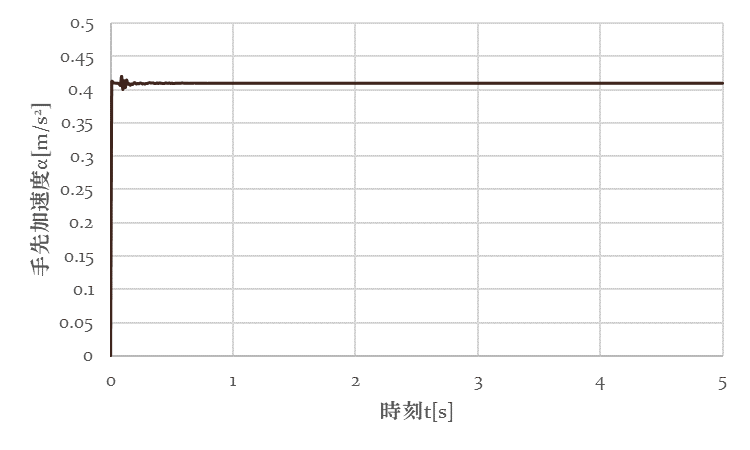
\includegraphics[width=12cm]{robocon/robot17.png}
  \caption{Harder Arm 手先加速度}
  \label{fig:Harder Arm 手先加速度}
\end{figure}
\begin{figure}[htbp]
  \centering
  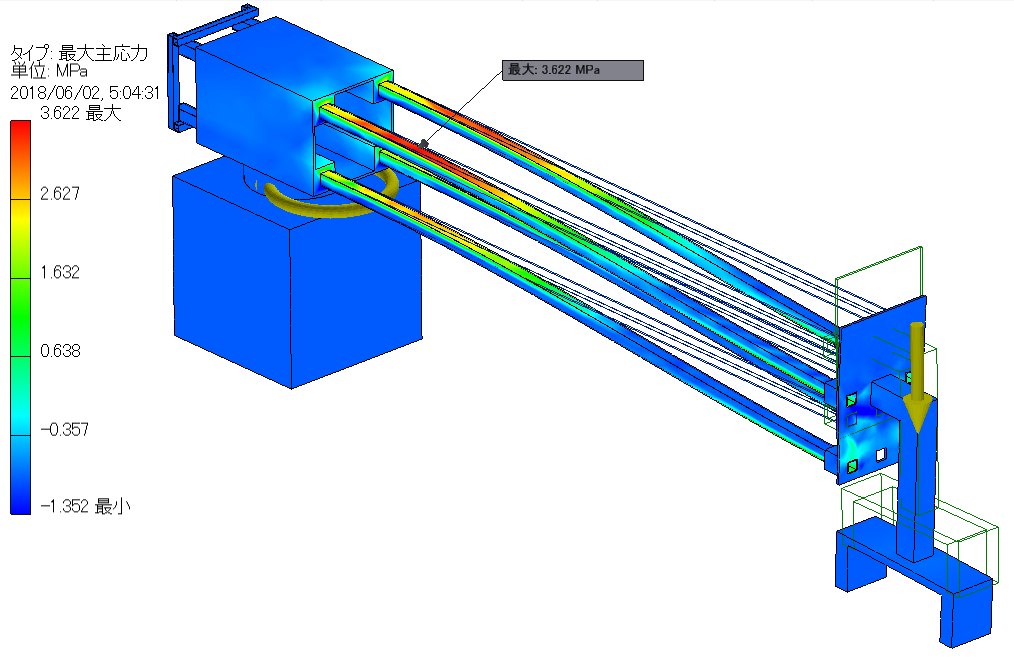
\includegraphics[width=12cm]{robocon/robot18.png}
  \caption{Harder Arm 最大主応力}
  \label{fig:Harder Arm 最大主応力}
\end{figure}
\begin{figure}[htbp]
  \centering
  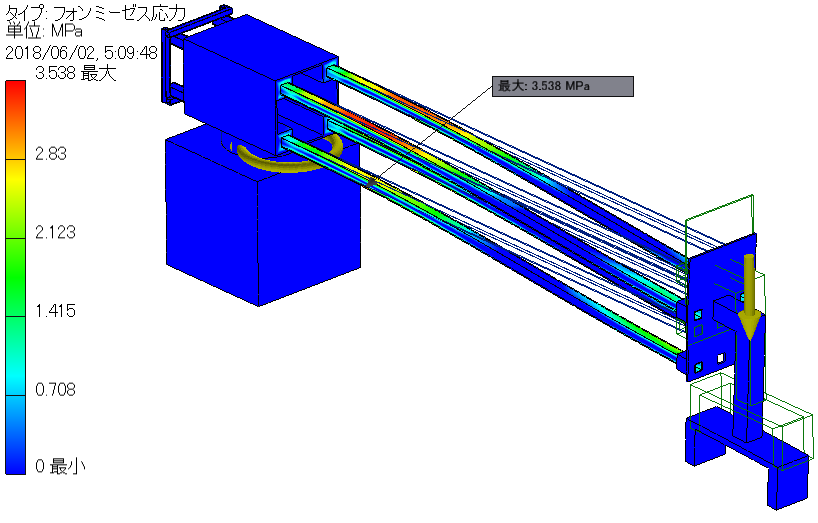
\includegraphics[width=12cm]{robocon/robot19.png}
  \caption{Harder Arm 最大フォンミーゼス応力}
  \label{fig:Harder Arm 最大フォンミーゼス応力}
\end{figure}
\begin{figure}[htbp]
  \centering
  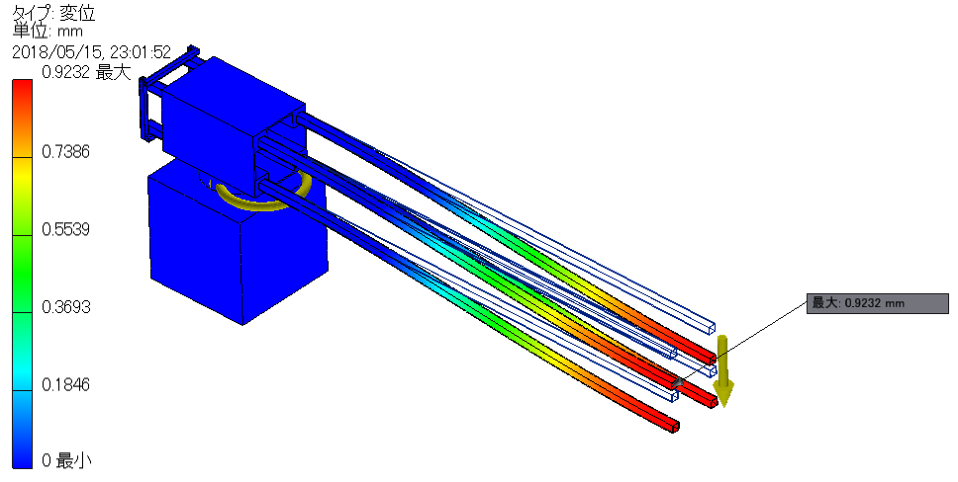
\includegraphics[width=13cm]{robocon/robot20.png}
  \caption{Harder Arm 変位}
  \label{fig:Harder Arm 変位}
\end{figure}
基準としたアームと重力方向の変位を抑えたアームの2つからパラメータを作成する. 左縦軸に高さ$h$を, 右縦軸に幅$b$をとり, 横軸に加速度$\alpha$をとってグラフを書くと, 図\ref{fig:alpha-h, alpha-b グラフ}のようになる. グラフの右下に交点を寄せつつ, 強度が要求を満たすように設計していく.
\begin{figure}[htbp]
  \centering
  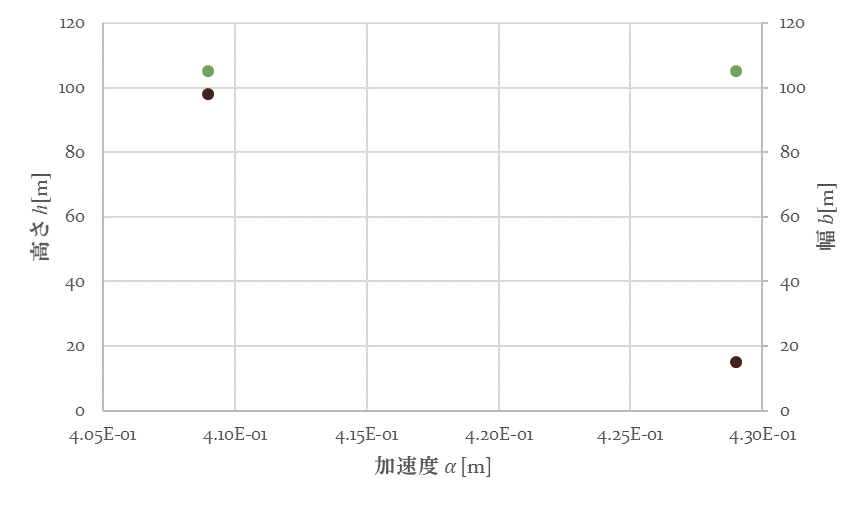
\includegraphics[width=13cm]{robocon/robot21.png}
  \caption{$\alpha-h, \alpha-b$グラフ}
  \label{fig:alpha-h, alpha-b グラフ}
\end{figure}

\clearpage
\subsection{最終形状}
最終的に, 以下に示す形状のリンクを設計した. Speedy Arm を図\ref{fig:Speedy Arm 形状と寸法}に示す. また, アセンブリを図\ref{fig:Speedy Arm アセンブリ図}に示す. 
このロボットアームを機構解析した結果, アーム先端に設定した手先座標系に関する手先角加速度, 手先角速度, 手先角度変化, 手先加速度が以下の図\ref{fig:Speedy Arm 手先角加速度}から図\ref{fig:Harder Arm 手先加速度2}までのグラフに示すように得られた. 
また, 構造解析結果として, 最大主応力, 最大フォンミーゼス応力, 変位が図\ref{fig:Speedy Arm最大主応力}, 図\ref{fig:Speedy Arm最大フォンミーゼス応力}, 図\ref{fig:Speedy Arm変位}のように得られた. 
その他に得られた数値もまとめて表\ref{tbl:Speedy Arm 解析結果}に示す.


\begin{table}[H]
  \centering
  \caption{Speedy Arm 解析結果}
  \label{tbl:Speedy Arm 解析結果}
  \begin{tabular}{|c|c|c|c|c|c|} \hline
  \begin{tabular}{c}質量\\$M\tani*{kg}$\end{tabular} & \begin{tabular}{c}角加速度\\$\ddot{q}$$\tani*{rad/s^2}$\end{tabular} & \begin{tabular}{c}加速度\\$\dot{q}$$\tani*{m/s}$\end{tabular} & \begin{tabular}{c}最大応力\\$\sigma\tani*{Pa}$\end{tabular} & \begin{tabular}{c}変位\\$\delta_z\tani*{m}$\end{tabular} & \begin{tabular}{c}重心の鉛直方向回り\\慣性モーメント\\$I_{S_0}\tani*{g mm^2}$\end{tabular} \\ \hline
$1.07$&$4.25\times 10^{-1}$&$4.25\times 10^{-1}$&$9.28\times 10^6$&$2.19\times 10^{-3}$&$1.02\times10^8$\\ \hline
  \end{tabular}
\end{table}


\begin{figure}[htbp]
  \centering
  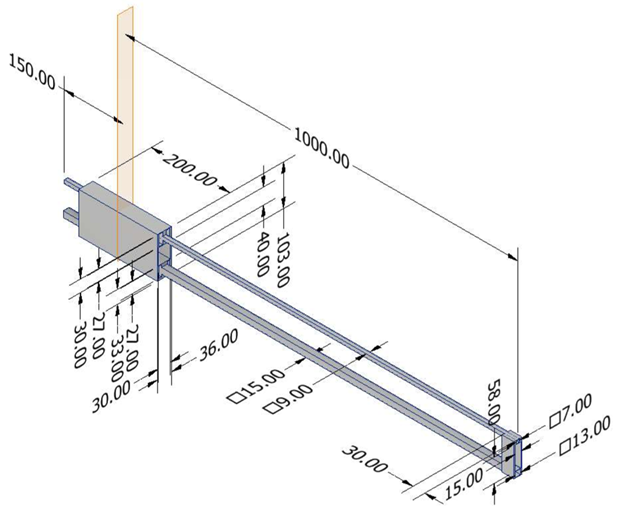
\includegraphics[width=10cm]{robocon/robot22.png}
  \caption{Speedy Arm 形状と寸法}
  \label{fig:Speedy Arm 形状と寸法}
\end{figure}
\begin{figure}[htbp]
  \centering
  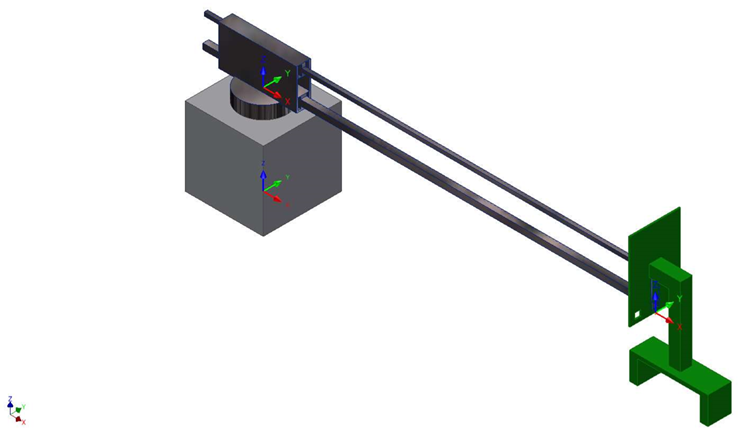
\includegraphics[width=8cm]{robocon/robot23.png}
  \caption{Speedy Arm アセンブリ図}
  \label{fig:Speedy Arm アセンブリ図}
\end{figure}
\begin{figure}[htbp]
  \centering
  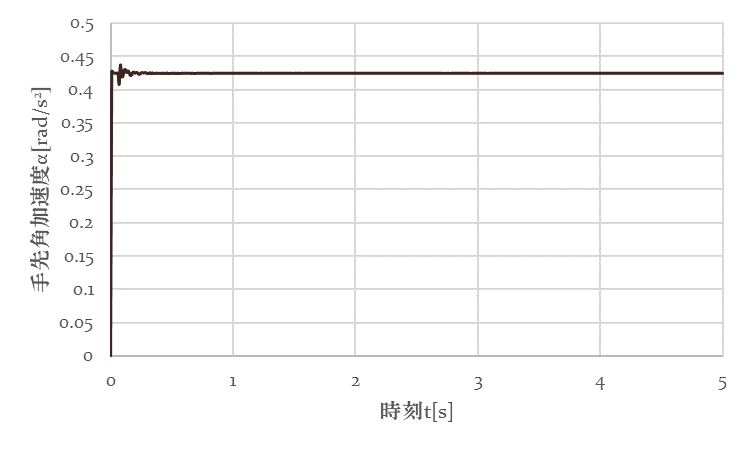
\includegraphics[width=10cm]{robocon/robot24.png}
  \caption{Speedy Arm 手先角加速度}
  \label{fig:Speedy Arm 手先角加速度}
\end{figure}
\begin{figure}[htbp]
  \centering
  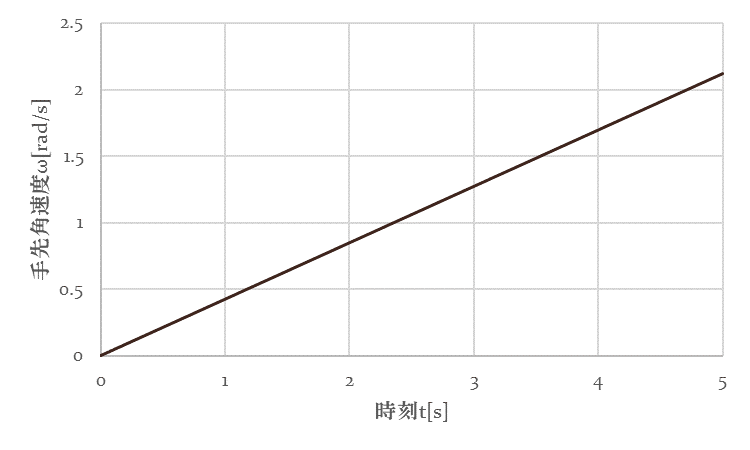
\includegraphics[width=10cm]{robocon/robot25.png}
  \caption{Speedy Arm 手先角速度}
  \label{fig:Speedy Arm 手先角速度}
\end{figure}
\begin{figure}[htbp]
  \centering
  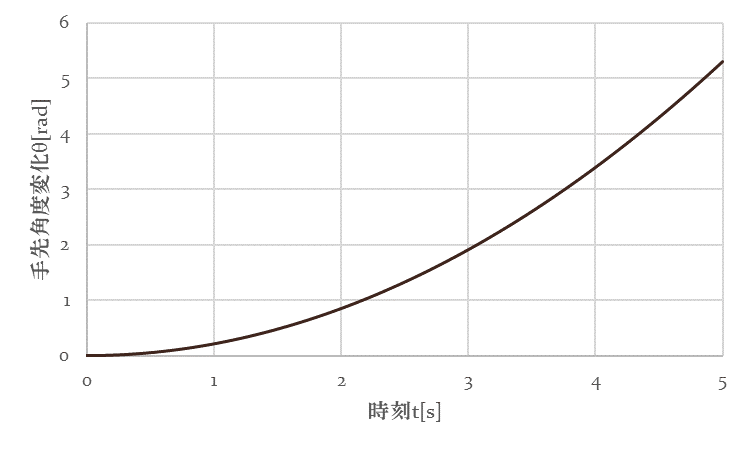
\includegraphics[width=10cm]{robocon/robot26.png}
  \caption{Speedy Arm 手先角度変化}
  \label{fig:Speedy Arm 手先角度変化}
\end{figure}
\begin{figure}[htbp]
  \centering
  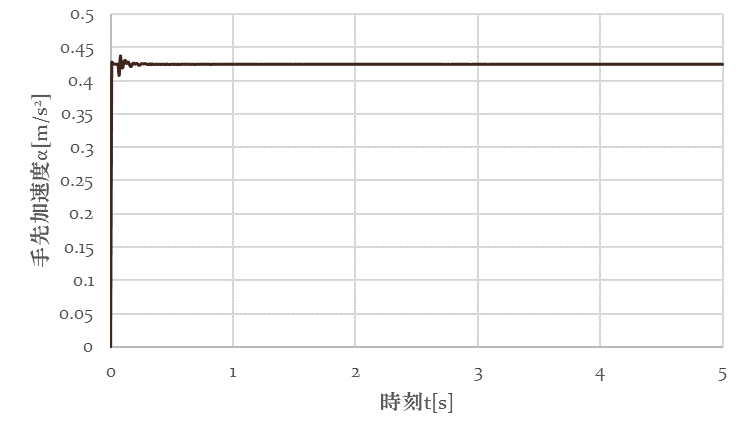
\includegraphics[width=10cm]{robocon/robot27.png}
  \caption{Harder Arm 手先加速度}
  \label{fig:Harder Arm 手先加速度2}
\end{figure}
\begin{figure}[htbp]
  \centering
  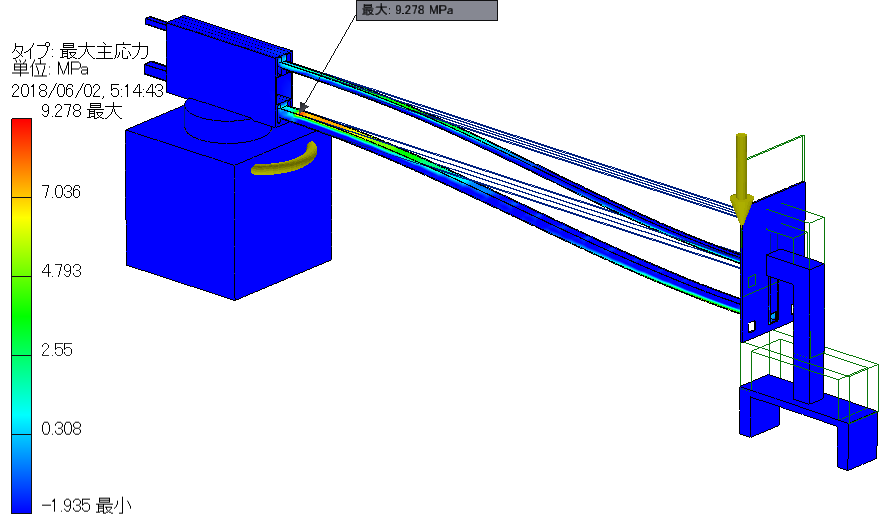
\includegraphics[width=10cm]{robocon/robot28.png}
  \caption{Speedy Arm最大主応力}
  \label{fig:Speedy Arm最大主応力}
\end{figure}
\begin{figure}[htbp]
  \centering
  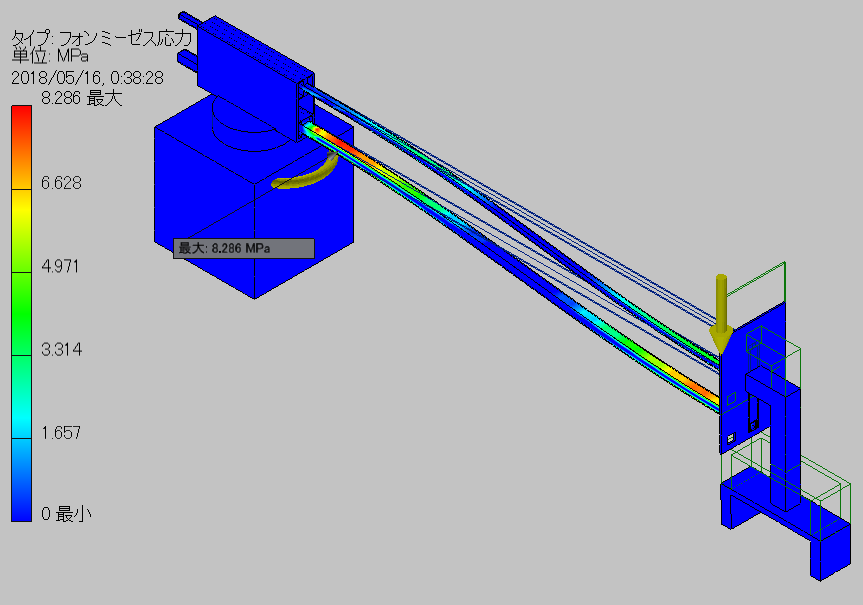
\includegraphics[width=10cm]{robocon/robot29.png}
  \caption{Speedy Arm最大フォンミーゼス応力}
  \label{fig:Speedy Arm最大フォンミーゼス応力}
\end{figure}
\begin{figure}[htbp]
  \centering
  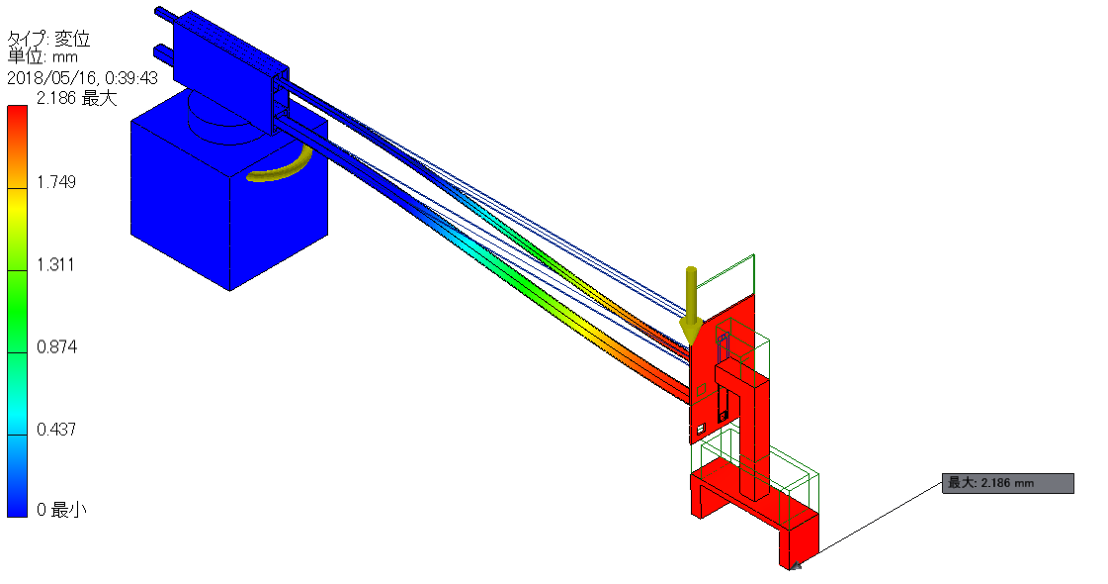
\includegraphics[width=10cm]{robocon/robot30.png}
  \caption{Speedy Arm変位}
  \label{fig:Speedy Arm変位}
\end{figure}
\subsection{確認}
解析解に基づいて得られた解が正しいと予想されるかどうかを確認する. 最終形状に適用した形状についての重要なパラメータとなる数値の理論値と数値解との比較を以て数値解の確認とする. 先ず, ロボットアームの角加速度, 角速度, 手先角加速度, 手先角速度, 手先速度を算出する式の重要なパラメータである慣性モーメントについて確かめる. 以降では, 簡略化のために理論解, 数値解をそれぞれ$I_S$,$I_{\tilde{S}}$,$I_{S_0}$と表記する. \ref{数式}項の式を用いて図\ref{fig:Speedy Arm 形状と寸法}に示す寸法を参照しながらアームの形状をいくつかの正の密度と負の密度を持つ複数の長方形に分割し, それぞれのアームの回転軸周りの慣性モーメントを計算すると

\begin{eqnarray}
  I_S&=&\sum_{i=1}^{n} \left\{ \frac{1}{12} \rho l_ib_ih_i(l_i^2+b_i^2)+\rho l_ib_ih_ix^2 \right\}\\
  &=&1.25\times10^8\tani*{g mm^2}
\end{eqnarray}
となる. また, 表\ref{tbl:Speedy Arm 解析結果}を参照して
\begin{eqnarray}
  I_S&=&I_{S_0}+Mx^2\\
  &=&1.26\times10^8\tani*{g mm^2}
\end{eqnarray}
ただし,$x$の値は$1.49\times10^2 \tani*{mm}$であり, 数値解による重心から回転軸までの距離である. 両数値はほぼ一致しており, 各数値解の値は正しいと言える.\par
最大応力については, 形状が複雑である為に応力の理論解を求めることは難しいので数値解を信用して評価する場合, 設計したすべての構造は応力については十分に要件を満たしていることは図\ref{fig:alpha-sigma_xグラフ}に示す通り, 明らかである. また, Speedy ArmはBasic Arm で達成できなかった変位の制限について,$2.19\times10^{-3} \tani*{m}$と十分に満たしており, 更にHarder Armより手先角加速度が大きいので, ロボットアームは十分に高速化され, 設計目標に達したと言える.

\begin{figure}[htbp]
  \centering
  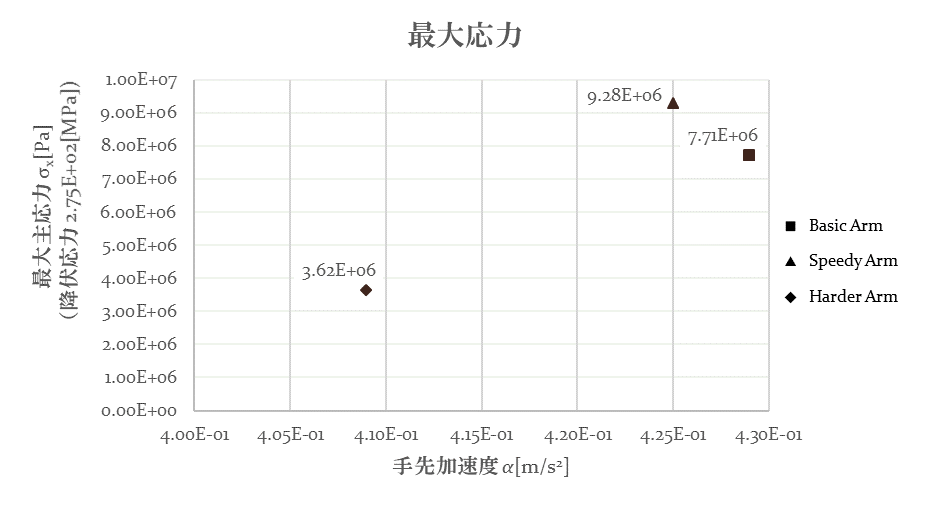
\includegraphics[width=13cm]{robocon/robot31.png}
  \caption{$\alpha-\sigma_x$グラフ}
  \label{fig:alpha-sigma_xグラフ}
\end{figure}
\begin{figure}[htbp]
  \centering
  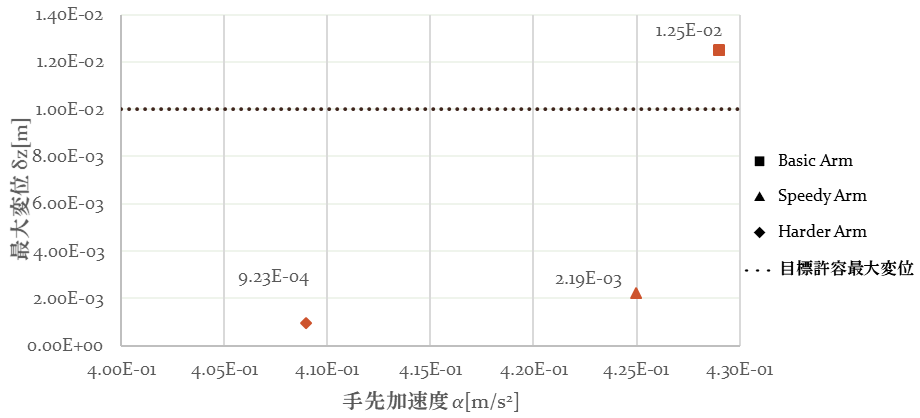
\includegraphics[width=13cm]{robocon/robot32.png}
  \caption{$\alpha-\delta_z$グラフ}
  \label{fig:alpha-delta_zグラフ}
\end{figure}
\section{終わりに}
\begin{itemize}
\item シミュレータを用いた設計を行う際には, どんな複雑な設計を行う前にもそのシミュレータをテストできる簡単なモデルを用意してテストをした方がよい.
\item リンクの高速化と剛性を求める場合は降伏応力のほかにも閾値を設けて設計する必要がある. 設計パラメータは何を目的に設計するかによって正確に選択する必要がある. 
\item ロボットアームを設計する際には重量がかさむものはロボットベースに近くなるように設計するか, 制御や機械要素による補償を施す必要がある
\item ある方向への変形による変位は, その方向に寸法を取る材料または構造の厚みが関係するので, アームの伸びに対していくらの変形を許容するかというパラメータは重要なパラメータの一つである.
\item CADソフトのファイル形式変換についての理解はシミュレーションソフトなどと連携した設計に欠かせない知識である. 無料のソフトウェアでも本格的な設計が可能なので積極的に使っていきたい. 今回は学生版のAutodesk Inventor 2018を用いて設計・構造解析などを行い, simXpertとのファイルの互換性についてある程度の理解を得た. また, 2018年度より本学で生徒のパソコンで利用できる包括ライセンスを導入したMATLABの拡張機能に含まれるシミュレーションアプリケーションと連携が可能であることが分かったので, 以後挑戦したいと思う. 
\end{itemize}

\section{付録}
計算した結果を用いて実際に以下に示すロボットアームを設計した. 
\begin{figure}[H]
  \centering
  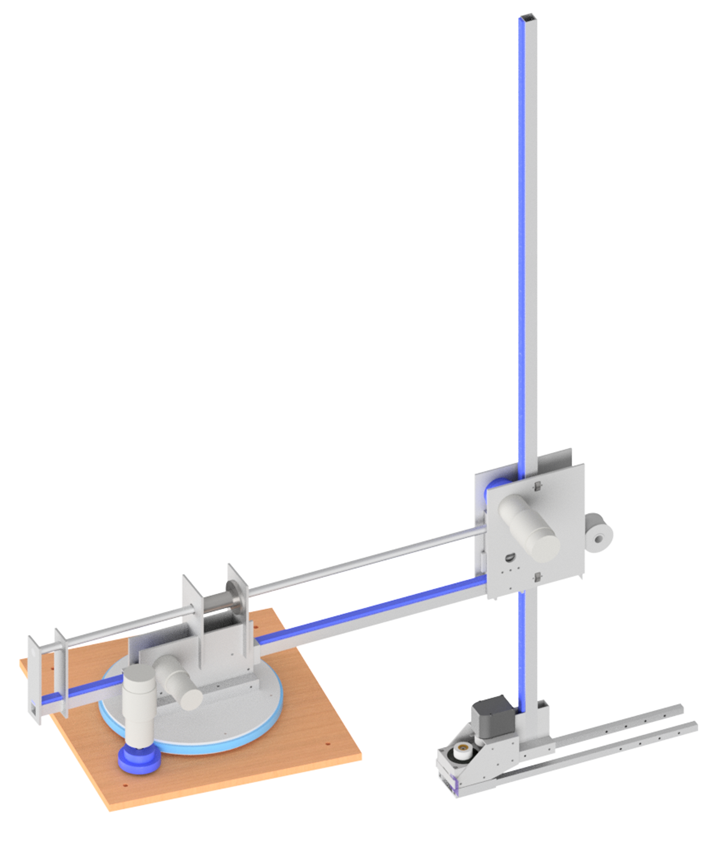
\includegraphics[width=10cm]{robocon/robot33.png}
\end{figure}

% \clearpage
%% 参考文献
\begin{thebibliography}{99}
  \item 著者, 本やページの名前, (URL), 出版社, 出版年.
  \item (複数ある場合は追加)
  \item @vuccaken, 物科研HP, \url{rp2017xy.starfree.jp}, 2019.
\end{thebibliography}


\end{document}
%
% ファイトだよ!
%
